\label{1.3.9}

The homogeneous coordinate ring is not an invariant under isomorphism. For example, let $X = \P^1$ an let $Y$ be the $2$-uple embedding of $\P^1$ in $\P^2$. Then $X \cong Y$ (\ref{1.3.4}). But show that $S(X) \not \cong S(Y)$.

\begin{proof}
    As explained in \ref{1.3.1}.c, $Y = Z(z^2 - xy)$. Then $S(Y) = k[x, y, z] / (z^2 - xy)$, which we claim is not isomorphic to $S(X) = k[x, y]$. First of all, the given map $S(Y) \longrightarrow S(X)$ via $x \mapstp x^2$, $y \mapsto y^2$, $z \mapsto xy$ is not as isomorphism, as its image is $k[x^2, xy, y^2] < k[x, y]$. But the question was not that this specific map is not an isomorphism, it is that no isomorphism at all can exist. First, consider the plot of $V(z^2 - xy) \subseteq \A^3$ below (figure \ref{fig1.3.2}).

    \begin{figure}[h]
        \centering
        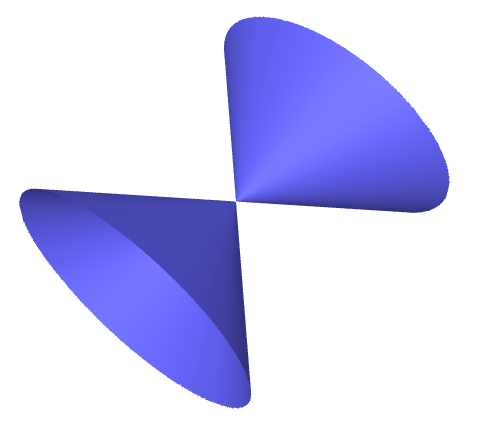
\includegraphics[scale=0.75]{double-cone}
        \caption{$V(z^2 - xy) \subseteq \A^3$}
        \label{fig1.3.2}
    \end{figure}

    There seems to be an issue at the origin. Again, this is a plot in $\R^3$ but we're only using it for ideas. As such, let's consider the localization of $S(Y)$ at the maximal ideal $\m = (x, y, z)$. First of all, note that every localization of $S(X) = k[x, y]$ by a maximal ideal is a regular local ring of dimension 2, so in particular the Zariski cotangent spaces $\mathfrak n/\mathfrak n^2$ are all 2 dimensional $k$ vector spaces, for $\mathfrak n$ a maximal ideal of $k[x, y]$.

    First of all, note that since $(z^2 - xy) \subseteq (x, y, z)$, $\m$ does indeed correspond to a maximal ideal of $S(Y)$. Specifically, this is $\m / (z^2 - xy)$. In fact, we have that $\m^2 \supseteq (z^2 - xy)$, so $\m^2$ corresponds to the ideal $\m^2 / (z^2 - xy)$. Now, these are ideals of $S(Y)$, so they are $S(Y)$ modules. Hence, they are also $k[x, y, z]$ modules. By the third isomorphism theorem, we have $\frac{\m / (z^2 - xy)}{\m^2 / (z^2 - xy)} \cong \m / \m^2$ as $k[x, y, z]$ modules. We can appeal to the general fact that $k[x, y, z]$ is a three dimensional regular ring, or just see directly that $(x, y, z) / (x, y, z)^2$ has $\{x, y, z\}$ as a $k$-basis (any higher order things are killed in the quotient). Thus, $\m / \m^2$ is three dimensional over $k$, so in particular $S(Y)$ localized at $\m$ is not a regular local ring. Thus, $S(Y) \not \cong S(X)$.

    My grasp on this connection is a bit tenuous, but the fact that the Zariski cotangent space at the origin of this variety is three dimensional, as opposed to the desired two dimensions, reflects the three tangent directions at the origin. Everywhere else on this variety is nice and smooth, so we'd expect a two dimensional regular local ring everywhere else.
\end{proof}
